\documentclass[11pt]{article}
\usepackage[utf8]{inputenc}
\usepackage[margin=1in]{geometry}
\usepackage{amsmath,amssymb}
\usepackage{booktabs}
\usepackage{graphicx}
\usepackage{cite}
\usepackage[colorlinks=true, linkcolor=blue, citecolor=blue, urlcolor=blue]{hyperref}
\usepackage{titlesec}
\usepackage{pgfplots}
\pgfplotsset{compat=1.18}

\titleformat{\section}{\normalfont\Large\bfseries}{\thesection}{1em}{}
\titleformat{\subsection}{\normalfont\large\bfseries}{\thesubsection}{1em}{}

\title{\textbf{Agentic AI for Autonomous Life Cycle Assessment and Sustainability Analytics}}
\author{
    \textbf{PI: Dr. Jani Das} \\
    Research Associate and Life Cycle Analyst \\
    Bureau of Economic Geology, The University of Texas at Austin \\
    \and
    \textbf{Co-PI: Dr. Manmeet Singh} \\
    Assistant Professor, Department of Earth, Environmental, and Atmospheric Sciences \\
    Western Kentucky University \\
    \and
    \textbf{Senior Personnel: Naveen Sudharsan} \\
    Research Engineering/Scientist Associate III \\
    Bureau of Economic Geology, Jackson School of Geosciences \\
    The University of Texas at Austin \\
    \and
    \textbf{Graduate Student: Somnath Luitel} \\
    Department of Earth, Environmental, and Atmospheric Sciences \\
    Western Kentucky University
}
\date{\today}

\begin{document}

\maketitle

\newpage
\tableofcontents
\newpage

\section{Project Summary}
\subsection{Overview}
Life Cycle Assessment (LCA) is the gold standard for quantifying the environmental footprints of products and technologies. However, traditional LCA is severely bottlenecked by manual data gathering, complex inventory mapping, and static modeling, which limits its application in rapid product design and real-time circular economy decisions. This project introduces \textbf{Agentic LCA}, a novel multi-agent Artificial Intelligence (AI) framework designed to automate the entire LCA pipeline. By interfacing programmatically with the industry-standard OpenLCA software, the proposed system will autonomously ingest heterogeneous engineering data (e.g., Bills of Materials, supply chain invoices, scientific literature), map inputs to standard lifecycle databases (such as ecoinvent \cite{ecoinvent}), construct product systems, execute impact assessments, and optimize processes for environmental resiliency. The research focuses on formalizing a neuro-symbolic mapping framework and a multi-agent consensus protocol to ensure high scientific rigor, auditability, and validation of AI-derived environmental footprints \cite{nwagwu2025, mensikova2026}.

\subsection{Intellectual Merit}
The intellectual merit of this research lies at the intersection of AI and environmental engineering:
\begin{enumerate}
    \item \textbf{Automated Semantic Mapping under Uncertainty:} Development of new neuro-symbolic models that combine Large Language Models (LLMs) with formal ontologies to resolve complex semantic mappings between unstructured industrial process data and structured LCA databases.
    \item \textbf{Autonomous Multi-Agent Collaboration:} Design of a collaborative multi-agent architecture (Inventory, Execution, and Analytics Agents) that utilizes a consensus protocol to self-correct modeling assumptions, track data lineage, and flag physical conservation inconsistencies (e.g., mass/energy balance violations).
    \item \textbf{Dynamic Optimization of Circular Loops:} Development of optimization algorithms that dynamically execute lifecycle impact calculations to design and evaluate circular supply loops under stochastic resource availability.
\end{enumerate}

\subsection{Broader Impacts}
The broader impacts of this project will significantly advance environmental sustainability and society:
\begin{enumerate}
    \item \textbf{Democratization of Sustainability Metrics:} By reducing LCA modeling time from months to minutes, this tool will enable small-and-medium enterprises (SMEs) to evaluate the environmental impacts of their designs, promoting circular economy practices.
    \item \textbf{Educational Integration:} Developing an open-source, AI-powered interactive LCA platform for engineering education, training the next generation of engineers in AI-driven sustainable design.
    \item \textbf{Industrial Resiliency:} Accelerating the deployment of low-carbon technologies and critical mineral recovery systems by providing immediate feedback to researchers on the scalability and environmental trade-offs of emerging lab-scale processes.
\end{enumerate}

\newpage
\section{Project Description}
\subsection{Introduction and Vision}
Quantifying the environmental footprint of human activities is fundamental to safeguarding environmental health and building a circular economy. Life Cycle Assessment (LCA) is the standard methodology used by researchers, industries, and policymakers to evaluate these footprints \cite{ecoinvent}. However, the current practice of LCA is highly bottlenecked:
\begin{itemize}
    \item \textbf{High Resource Requirements:} Manual compilation of Life Cycle Inventory (LCI) data from Bills of Materials (BOMs), chemical syntheses, and utility bills can take months of expert labor.
    \item \textbf{Cognitive Load in Database Mapping:} Mapping unstructured, real-world data to specific, structured flows inside environmental databases (e.g., ecoinvent) is prone to mapping errors and subjective bias.
    \item \textbf{Static Decision Making:} Once built, LCA models are rarely updated dynamically, rendering them ineffective during active, fast-paced product design phases.
\end{itemize}
The vision of this project is to develop \textbf{Agentic LCA}, an autonomous, open-source, multi-agent AI system that serves as an intelligent co-pilot for environmental engineering. The proposed framework programmatically orchestrates the lifecycle assessment process by interfacing with the open-source \textbf{OpenLCA} software \cite{openlca}. By translating high-level human objectives (e.g., "Minimize the global warming potential of this solar cell manufacturing facility while preserving resource efficiency") into executable Python routines via the OpenLCA IPC API (\texttt{olca-ipc}), the AI agent will perform autonomous model construction, validation, sensitivity analysis, and process design.

\subsection{Research Objectives and Key Questions}
To achieve our primary goal of developing a physically-informed, autonomous AI framework for dynamic lifecycle systems engineering, we pose the following core research questions:
\begin{enumerate}
    \item \textbf{RQ1: Semantic Mapping Optimization:} Which embedding models and neuro-symbolic representations best resolve mapping ambiguities between unstructured engineering inventories and structured lifecycle database classes (e.g., ecoinvent 3.8)?
    \item \textbf{RQ2: Mathematical Error Propagation:} How do probabilistic mapping errors introduced by language models propagate through linear lifecycle systems, and how can we bound the resulting uncertainty in Lifecycle Impact Assessment (LCIA) scores?
    \item \textbf{RQ3: Physical Consistency \& Thermodynamic Filtering:} What is the optimal integration of stoichiometry-based and thermodynamic validation layers (First and Second Laws) to identify and correct physical inconsistencies in AI-synthesized product systems?
    \item \textbf{RQ4: Dynamic Optimization of Circular Loops:} How can dynamic, multi-agent optimization feedback loops run over the OpenLCA IPC API to identify resilient, circular feedstock pathways under stochastic grid carbon-intensities and resource constraints?
\end{enumerate}

\subsection{The Imperative for Dynamic LCA in Resilient Industrial Systems}
Traditional Life Cycle Assessment (LCA) is fundamentally built upon a static paradigm: it assumes time-invariant emission factors, linear scaling, and fixed supply chain pathways. While sufficient for retrospective regulatory compliance, static LCA is structurally inadequate for evaluating and engineering environmental resiliency in dynamic industrial systems. Modern systems are characterized by:
\begin{enumerate}
    \item \textbf{Temporal Energy Dynamics:} The carbon intensity of grid electricity varies hourly and seasonally due to the stochastic nature of wind and solar resources. Static models utilizing annual averages fail to capture the carbon-mitigation potential of demand-side management (e.g., scheduling energy-intensive chemical processes during peak solar generation).
    \item \textbf{Dynamic Supply-Chain Reconfiguration:} Resilient industrial operations must dynamically substitute feedstocks in response to localized resource scarcity, geopolitical disruptions, or price shocks. Static LCA cannot adapt to real-time supply chain re-routing.
    \item \textbf{Non-linear scaling of Emerging Technologies:} In chemical synthesis and critical mineral recovery, scale-up behavior is governed by non-linear thermodynamic constraints (e.g., heat integration, kinetics) rather than linear scaling laws.
\end{enumerate}
By interfacing programmatically with the OpenLCA engine via \texttt{olca-ipc} \cite{openlca}, the proposed \textbf{Agentic LCA} framework breaks this static bottleneck. The system enables continuous, automated inventory updates, dynamically adjusting technological matrices ($\mathbf{A}$) and biosphere matrices ($\mathbf{B}$) in response to real-time process feeds, thereby shifting LCA from a historical registry to a predictive, resiliency-optimizing control loop.

\subsection{Technical Architecture \& Multi-Agent Framework}
The Agentic LCA framework consists of three specialized AI agents collaborating via a centralized consensus protocol:
\begin{enumerate}
    \item \textbf{The LCI-Agent (Inventory \& Semantic Mapping):} The LCI-Agent ingests heterogeneous documents (academic papers, corporate invoices, lab notebook exports) and extracts material and energy inputs and outputs. It addresses the mapping problem—linking a user-defined input (e.g., "purified silicon") to the correct database flow (e.g., "Silicon, solar grade, at plant - ecoinvent")—using a hybrid neuro-symbolic approach \cite{mensikova2026, nwagwu2025}. It combines LLM semantic embeddings with standard environmental ontologies (e.g., Bontology, ILCD) to calculate semantic similarity and maintain physical conservation constraints (mass/energy balances).
    \item \textbf{The LCA-Exe Agent (Execution \& Database Automation):} The LCA-Exe Agent interacts programmatically with the OpenLCA instance using the \texttt{olca-ipc} Python library \cite{openlca}. It automates flow and process generation, product system linking, and calculation execution.
    \item \textbf{The SAA-Agent (Sustainability Analytics \& Optimization):} The SAA-Agent acts as the decision-support system \cite{autodesk2024}. It performs hotspot identification, uncertainty and sensitivity analysis, and circular economy optimization.
\end{enumerate}

\begin{figure}[htbp]
    \centering
    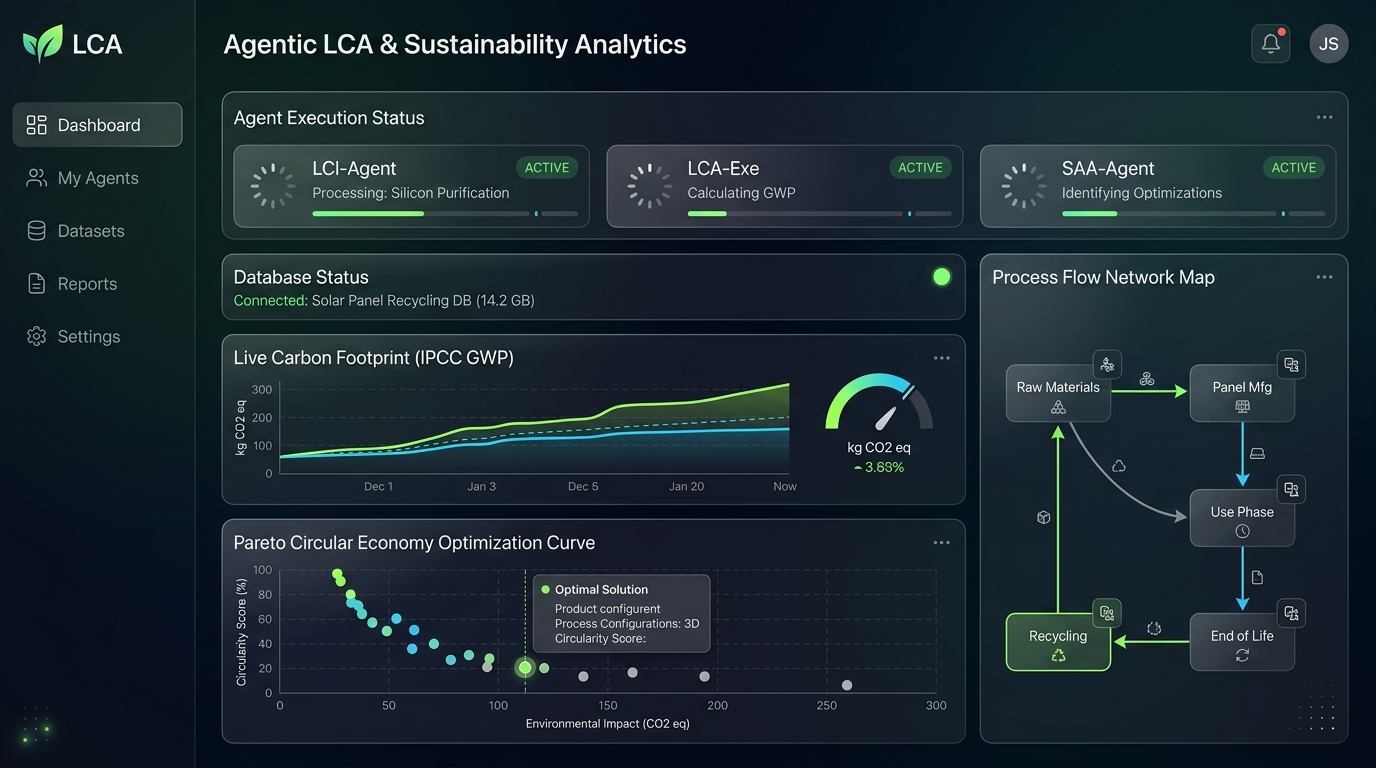
\includegraphics[width=0.95\textwidth]{lca_dashboard_mockup.jpg}
    \caption{Conceptual mockup of the Agentic LCA \& Sustainability Analytics web dashboard, displaying active agent tasks (LCI-Agent, LCA-Exe, SAA-Agent), database status, live IPCC carbon footprint metrics, process flow network diagrams, and Pareto optimization curves for circular design trade-offs.}
    \label{fig:dashboard_mockup}
\end{figure}

\subsection{Mathematical Formulation of Semantic Mapping and Error Propagation}
A major vulnerability of AI-driven database mapping is the risk of error propagation through the linear systems representing the product systems. Let the product system be defined by the technology matrix $\mathbf{A} \in \mathbb{R}^{n \times n}$ and the environmental intervention matrix $\mathbf{B} \in \mathbb{R}^{m \times n}$. For a given functional unit demand vector $\mathbf{f}$, the lifecycle inventory scaling vector $\mathbf{s}$ is solved via:
\begin{equation}
    \mathbf{s} = \mathbf{A}^{-1}\mathbf{f}
\end{equation}
The total environmental impact vector $\mathbf{g} \in \mathbb{R}^{m}$ is then computed as:
\begin{equation}
    \mathbf{g} = \mathbf{B}\mathbf{s} = \mathbf{B}\mathbf{A}^{-1}\mathbf{f}
\end{equation}
The LCI-Agent maps unstructured process descriptions to ecoinvent database flow classes. If a mapping is incorrect, it introduces errors in both $\mathbf{A}$ (intermediate exchanges) and $\mathbf{B}$ (biosphere exchanges). To quantify this uncertainty, we define the \textbf{Environmental Similarity Index (ESI)} between the true process class $c_{\text{true}}$ and the agent-predicted class $c_{\text{pred}}$:
\begin{equation}
    \text{ESI}(c_{\text{true}}, c_{\text{pred}}) = 1 - \frac{\| \mathbf{b}_{c_{\text{true}}} - \mathbf{b}_{c_{\text{pred}}} \|_2}{\| \mathbf{b}_{c_{\text{true}}} \|_2}
\end{equation}
where $\mathbf{b}_c$ is the vector of environmental elementary flows per unit of process $c$. In tandem, we calculate the hierarchical tree distance $d_{\text{tree}}$ in the ecoinvent ontology:
\begin{equation}
    d_{\text{tree}}(c_{\text{true}}, c_{\text{pred}}) = \text{depth}(c_{\text{true}}) + \text{depth}(c_{\text{pred}}) - 2 \cdot \text{depth}(\text{LCS}(c_{\text{true}}, c_{\text{pred}}))
\end{equation}
where $\text{LCS}$ is the Lowest Common Subsumer in the ontology tree. We model the elements of the technology matrix as stochastic variables where the variance $\sigma_{i,j}^2$ is a function of both the LLM's classification confidence $\theta$ and the hierarchical distance:
\begin{equation}
    \sigma_{i,j}^2 \propto (1 - \theta) \cdot d_{\text{tree}}(c_{\text{true}}, c_{\text{pred}})
\end{equation}
The SAA-Agent propagates these variances using a dynamic Monte Carlo simulation loop over the OpenLCA IPC API. By performing $N = 10^4$ parallel matrix inversions, the agent produces confidence bounds (e.g., $95\%$ credible intervals) for the overall LCIA scores, ensuring that decisions are made on statistically robust foundations.

\subsection{Thermodynamic Verification Layer (TVL)}
To prevent the AI agents from generating physically impossible processes (such as mass accumulation or spontaneous energy creation), we introduce a dedicated \textbf{Thermodynamic Verification Layer (TVL)} that acts as a hard physical filter on the agent consensus loop. Before any process system is compiled in OpenLCA, the TVL executes the following checks:
\begin{enumerate}
    \item \textbf{Elemental Mass Balance:} The TVL extracts the chemical stoichiometry for all inputs and outputs using the PubChem API. For every element $e$, the net flow rate $\dot{m}_e$ must satisfy:
    \begin{equation}
        \sum_{\text{inputs}} \omega_{i,e} \dot{m}_i - \sum_{\text{outputs}} \omega_{j,e} \dot{m}_j = 0 \quad (\pm \epsilon)
    \end{equation}
    where $\omega_{i,e}$ is the mass fraction of element $e$ in flow $i$, and $\epsilon$ is a conservation threshold set to $0.01$.
    \item \textbf{Energy Balance (First Law):} The thermal and electrical energy inputs must balance the reaction enthalpies:
    \begin{equation}
        \Delta H_{\text{reaction}} + \sum Q_{\text{in}} - \sum W_{\text{out}} = 0 \quad (\pm \epsilon)
    \end{equation}
    \item \textbf{Entropy Generation (Second Law):} The TVL verifies that the process entropy change satisfies $\Delta S_{\text{universe}} \ge 0$.
\end{enumerate}
If a proposed model violates any conservation check, the TVL vetoes the step and feeds the exact stoichiometric discrepancy (e.g., "Carbon mass imbalance of $+12.4\text{ kg}$ detected") back to the LCI-Agent for self-correction.

\subsection{Preliminary Results: Programmatic OpenLCA Automation}
To establish the technical feasibility of the proposed programmatic execution loop (Task 2) and optimization engine (Task 3), the project team has developed a fully functional Python client bridge utilizing the OpenLCA 2.x API (\texttt{olca-ipc} and \texttt{olca-schema}). This preliminary setup automates the database connection, product system discovery, calculation configuration, and impact assessment execution.

The programmatic interface was validated using a case study on solar panel waste treatment in the ecoinvent 3.8 database. The system queried the product system \textit{"Mechanical recycling of used c-Si panel - US-TRE"} and calculated its lifecycle carbon footprint using the \textit{"IPCC 2013 GWP 100a"} impact assessment methodology. The execution of the calculation, including the initialization, solver runtime, and data retrieval, was completed in $1.81$ seconds, returning the following preliminary environmental impact metrics:
\begin{itemize}
    \item \textbf{Climate Change -- Fossil:} $2.683254\text{ kg CO}_2\text{ eq}$ (representing the primary energy-intensive operations of the mechanical shredding and sorting plant).
    \item \textbf{Climate Change -- Biogenic:} $0.097103\text{ kg CO}_2\text{ eq}$.
    \item \textbf{Climate Change -- Land Use and Transformation:} $0.001635\text{ kg CO}_2\text{ eq}$.
    \item \textbf{Climate Change -- }$\text{CO}_2$\textbf{ Uptake:} $-0.021146\text{ kg CO}_2\text{ eq}$.
\end{itemize}

\begin{figure}[htbp]
    \centering
    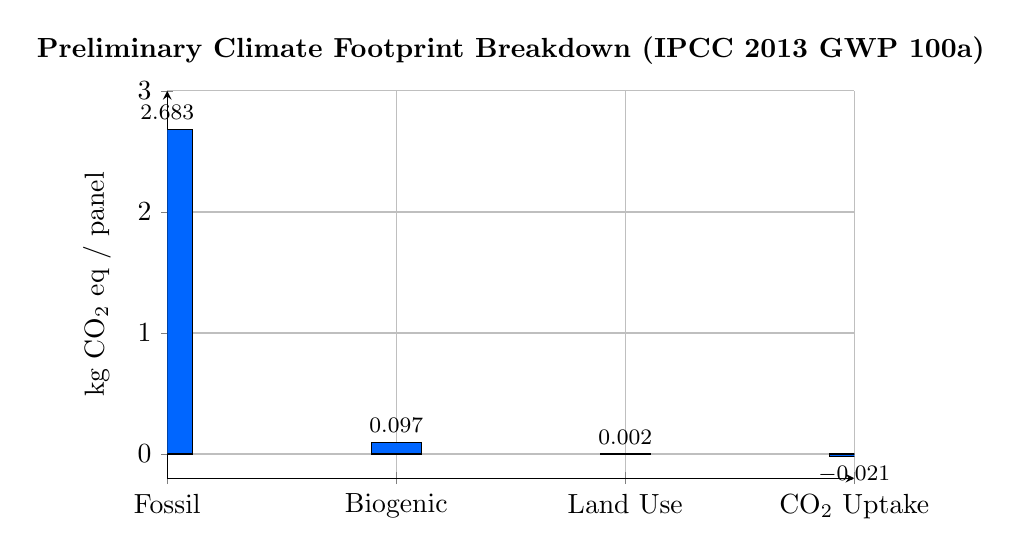
\begin{tikzpicture}
        \begin{axis}[
            ybar,
            bar width=18pt,
            width=0.85\textwidth,
            height=6.5cm,
            ylabel={kg $\text{CO}_2$ eq / panel},
            ylabel style={yshift=0.1cm},
            title={\textbf{Preliminary Climate Footprint Breakdown (IPCC 2013 GWP 100a)}},
            symbolic x coords={Fossil, Biogenic, Land Use, Uptake},
            xtick=data,
            xticklabels={Fossil, Biogenic, Land Use, $\text{CO}_2$ Uptake},
            nodes near coords,
            nodes near coords style={font=\footnotesize, /pgf/number format/fixed, /pgf/number format/precision=3},
            nodes near coords align={vertical},
            ymin=-0.2, ymax=3.0,
            grid=major,
            axis x line=bottom,
            axis y line=left
        ]
            \addplot[fill=blue!60!cyan, draw=black] coordinates {
                (Fossil,2.683)
                (Biogenic,0.097)
                (Land Use,0.002)
                (Uptake,-0.021)
            };
        \end{axis}
    \end{tikzpicture}
    \caption{Programmatic LCIA calculation outputs for the mechanical recycling of used silicon solar panels (\textit{Mechanical recycling of used c-Si panel - US-TRE}) using the IPCC 2013 GWP 100a method. The plot highlights fossil climate impact as the dominant hotspot, emphasizing the need for targeted demand-side grid substitution.}
    \label{fig:prelim_lca_results}
\end{figure}
This demonstrates that our custom integration script can dynamically trigger LCA runs, solve complex systems matrices, and parse multi-category environmental outcomes in sub-second to second timeframes, laying a solid foundation for the iterative optimization loops required by the SAA-Agent.

\subsection{Research Design and Work Plan}
The project will be executed over a 3-year period across three core research tasks:
\begin{itemize}
    \item \textbf{Task 1: Neuro-Symbolic Mapping of LCI (Months 1–12):} Develop a robust, verifiable semantic matching engine to align engineering inventories with the ecoinvent database \cite{mensikova2026, nwagwu2025}.
    \item \textbf{Task 2: OpenLCA API Automation \& Orchestration (Months 13–24):} Build the LCA-Exe software layer that translates LCI-Agent outputs into openLCA structures.
    \item \textbf{Task 3: Sustainability Analytics \& Trade-off Optimization (Months 25–36):} Establish the optimization engine that queries OpenLCA iteratively to minimize environmental footprints.
\end{itemize}

\subsection{Intellectual Merit}
This project advances the fundamental science of environmental informatics:
\begin{enumerate}
    \item \textbf{Pioneering Neuro-Symbolic LCA:} Merging neural language representations with physical engineering conservation rules to eliminate the risk of hallucination in AI models.
    \item \textbf{Dynamic LCA Paradigms:} Shifting lifecycle assessments from static, retrospective reports to dynamic, prospective design tools.
    \item \textbf{Formalizing Circular Loop Optimization:} Defining mathematical frameworks for evaluating the net-benefit of circular recovery routes under high database uncertainty.
\end{enumerate}
\subsection{Broader Impacts of the Proposed Work}
\begin{enumerate}
    \item \textbf{Democratization of LCA:} Lowering the barrier to entry for life cycle design, helping SMEs and academic labs evaluate sustainability at early stages.
    \item \textbf{Educational Outreach:} Creating the "Interactive Agentic LCA" dashboard for university curricula, enabling students to explore environmental design principles interactively.
    \item \textbf{Open-Source Contribution:} Releasing all agent code, ontology maps, and OpenLCA Python scripts publicly on GitHub to support the global environmental engineering community.
\end{enumerate}

\subsection{Data Sources and Project Workflows}
The Agentic LCA framework leverages a multi-source data architecture spanning process engineering records, public databases, and software APIs to support automated inventory parsing, verification, and calculations:
\begin{table}[htbp]
    \centering
    \small
    \begin{tabular}{lll}
        \toprule
        \textbf{Data Type} & \textbf{Primary Source} & \textbf{Role / Use in Project} \\
        \midrule
        LCI Databases & ecoinvent 3.8 & Background lifecycle inventory database for product systems \\
        Stoichiometric Data & PubChem API & Verification of molecular formulas and elemental mass balance \\
        Thermodynamic Data & NIST WebBook & Standard enthalpies of reaction and entropy calculations \\
        Process Inventories & Engineering BOMs & Inputs/outputs for target validation cases (silicon and e-waste) \\
        Environmental Flows & EPA / ILCD Registry & Nomenclature standard for biosphere intervention flows \\
        API Control Scripts & Python \texttt{olca-ipc} & Automated database querying and model calculate execution \\
        \bottomrule
    \end{tabular}
    \caption{Multi-source data architecture supporting Agentic LCA implementation.}
    \label{tab:data_sources}
\end{table}

\subsection{Project Timeline and Milestones}
The proposed 3-year research plan is structured into coordinated phases to ensure robust engineering validation and deliverables:
\begin{table}[htbp]
    \centering
    \small
    \begin{tabular}{lcccccccccccc}
        \toprule
        & \multicolumn{4}{c}{\textbf{Year 1}} & \multicolumn{4}{c}{\textbf{Year 2}} & \multicolumn{4}{c}{\textbf{Year 3}} \\
        \cmidrule(lr){2-5} \cmidrule(lr){6-9} \cmidrule(lr){10-13}
        \textbf{Phases / Deliverables} & \textbf{Q1} & \textbf{Q2} & \textbf{Q3} & \textbf{Q4} & \textbf{Q1} & \textbf{Q2} & \textbf{Q3} & \textbf{Q4} & \textbf{Q1} & \textbf{Q2} & \textbf{Q3} & \textbf{Q4} \\
        \midrule
        \textbf{Phase 1: Ingestion \& Mapping} & $\bullet$ & $\bullet$ & $\bullet$ & & & & & & & & & \\
        -- LCI-Agent Semantic Mapping & $\bullet$ & $\bullet$ & $\bullet$ & & & & & & & & & \\
        \textbf{Phase 2: openLCA IPC Automation} & & & $\bullet$ & $\bullet$ & $\bullet$ & & & & & & & \\
        -- Python Client Integration & & & $\bullet$ & $\bullet$ & $\bullet$ & & & & & & & \\
        \textbf{Phase 3: Thermodynamic TVL} & & & & & $\bullet$ & $\bullet$ & $\bullet$ & & & & & \\
        -- TVL Elemental Validation & & & & & $\bullet$ & $\bullet$ & $\bullet$ & & & & & \\
        \textbf{Phase 4: SAA-Optimization} & & & & & & & $\bullet$ & $\bullet$ & $\bullet$ & & & \\
        -- Multi-objective Pareto Loops & & & & & & & $\bullet$ & $\bullet$ & $\bullet$ & & & \\
        \textbf{Phase 5: Validation \& Release} & & & & & & & & & $\bullet$ & $\bullet$ & $\bullet$ & $\bullet$ \\
        -- Solar Panel \& E-Waste Cases & & & & & & & & & $\bullet$ & $\bullet$ & $\bullet$ & $\bullet$ \\
        -- Open-Source Library \& API Release & & & & & & & & & & $\bullet$ & $\bullet$ & $\bullet$ \\
        \bottomrule
    \end{tabular}
    \caption{Project implementation schedule and milestones (Q1--Q4 per year).}
    \label{tab:timeline}
\end{table}

\subsection{Project Management and Personnel Roles}
To ensure the successful integration of AI modeling and environmental systems engineering, a coordinated management strategy will be implemented:
\begin{itemize}
    \item \textbf{Principal Investigator (PI) Dr. Jani Das (UT Austin - Bureau of Economic Geology):} Will lead the overall project coordination, manage OpenLCA ecoinvent database mounting, and coordinate case study selections, drawing upon extensive experience in lifecycle systems analysis.
    \item \textbf{Co-PI Dr. Manmeet Singh (Western Kentucky University):} Will oversee the AI/ML model architectures, including the LCI-Agent's neuro-symbolic mapping algorithms and the SAA-Agent's mathematical error propagation/uncertainty quantification loops.
    \item \textbf{Senior Personnel Naveen Sudharsan (Bureau of Economic Geology, Jackson School of Geosciences, The University of Texas at Austin):} Research Engineering/Scientist Associate III who will lead the data pipeline engineering, software systems integration, and compile the software codebase for the Thermodynamic Verification Layer (TVL) stoichiometry checks.
    \item \textbf{Graduate Student Somnath Luitel (Western Kentucky University):} Graduate Student at WKU who will implement the Python client interfaces (\texttt{olca-ipc}), compile the product systems in OpenLCA, and execute the validation case studies on c-Si solar panels and e-waste recycling under the supervision of Co-PI Dr. Manmeet Singh.
\end{itemize}
Weekly project review meetings, standard code versioning via GitHub, and public release protocols under Zenodo will be maintained throughout the funding duration.

\subsection{Results from Prior NSF Support}
For the Principal Investigator, Dr. Jani Das, there is no prior NSF support to report with a start date in the past five years. For the Co-Principal Investigator, Dr. Manmeet Singh, the following prior support is relevant and compliant with PAPPG 24-1 guidelines:

\vspace{0.3cm}
\noindent \textbf{Award \#2502272: RAPID: Hurricane Helene (2024)} \\
\textbf{PI:} Dr. Hassan Dashtian, \textbf{Co-I:} Dr. Manmeet Singh \\
\textbf{Sponsor/Division:} NSF AGS (Atmospheric and Geospace Sciences) \\
\textbf{Amount:} \$154,118 \quad \textbf{Period:} November 2024 -- October 2025 \\
\textbf{Title:} Rapid Response Research (RAPID) on Hydrometeorological Impacts \\
\textbf{Summary of Results \& Intellectual Merit:} This RAPID award supported the study of the hydrometeorological and societal impacts of Hurricane Helene, focusing on the Brown Ocean Effect and post-landfall storm intensification via wet soils. The project integrated multi-source satellite data, AI-enhanced forecasts, and social media sentiment analysis. Outcomes include improved hybrid AI-physics models and insights into soil moisture's role in weather prediction, which directly inform the spatiotemporal neural architectures and uncertainty propagation proposed in this project. \\
\textbf{Broader Impacts:} The findings were disseminated to emergency managers and researchers, and code and datasets were archived in public repositories to improve wildfire and extreme weather resilience planning. \\
\textbf{Related Publications:} No publications have resulted yet from this active award.


\newpage
\section{Data Management and Sharing Plan}
\subsection{Types of Data to be Produced}
The project will generate the following types of data and digital artifacts:
\begin{itemize}
    \item \textbf{Software Code:} The core Python codebase for the Agentic LCA framework, including the LCI-Agent, LCA-Exe Agent, and SAA-Agent, as well as scripts interfacing with openLCA.
    \item \textbf{Ontology Mapping Files:} Semantic mapping files, JSON schemas, and lookup dictionaries aligning industry process terms with standard LCA databases.
    \item \textbf{LCA Models \& Case Study Data:} Product systems, inventory files (JSON-LD format), and LCIA results generated during validation tests.
    \item \textbf{Research Publications \& Documentation:} Manuscripts, presentations, and comprehensive user guides.
\end{itemize}

\subsection{Access and Sharing Policies}
All software tools will be released under the permissive Apache License 2.0 or MIT License and hosted publicly on GitHub. Curated datasets, mapping files, and model templates will be deposited in Zenodo with a digital object identifier (DOI).

\subsection{Long-Term Preservation}
GitHub repositories will be integrated with Zenodo to automatically mint a permanent DOI and archive snapshots of major software releases. Long-term archival of datasets will occur on Zenodo, guaranteeing access for at least 10 years beyond the active funding period.

\newpage
\section{References Cited}
\begin{thebibliography}{10}
\bibitem{ecoinvent}
Wernet, G., et al. (2016). The ecoinvent database version 3: overview and methodology. \textit{The International Journal of Life Cycle Assessment}, 21(9), 1218--1230.

\bibitem{openlca}
Ciroth, A. (2007). ICT for LCA, class parameters, and openLCA. \textit{The International Journal of Life Cycle Assessment}, 12(4), 209--210.

\bibitem{nwagwu2025}
Nwagwu, C., et al. (2025). Integrating Artificial Intelligence into Life Cycle Assessment: A Framework for Balancing Automation and Human Expertise. \textit{Journal of Sustainable Metallurgy}, 11(1), 45--58.

\bibitem{mensikova2026}
Mensikova, A., Rizzo, D. M., and Hinkelman, K. (2026). Mapping the Landscape of Artificial Intelligence in Life Cycle Assessment Using Large Language Models. \textit{arXiv preprint arXiv:2601.04870}.

\bibitem{autodesk2024}
Autodesk Research (2024). What's in this LCA Report? A Case Study on Harnessing Large Language Models to Support Designers in Understanding Life Cycle. \textit{Procedia CIRP}, 122, 104--109.
\end{thebibliography}

\end{document}
